% !TeX root = kalpasthana-book.tex

\chapter{Kalpasthāna: Introduction}

The \emph{Kalpasthāna} of the \emph{Compendium of Suśruta} is one of
the most important treatises on toxicology surviving from the ancient
world.\footnote{\citet{liu-2021} provides a valuable overview of
    poison treatises in the ancient world, inexplicably omitting mention
    of the \emph{Kalpasthāna}.} Other treatises, such as the
    \emph{\textgreek{θηριακά}} (\emph{On Wild Animals}) and
    \emph{\textgreek{Ἀλεξίφαρμακα}} (\emph{Antidotes}) of Nicander of
    Colophon (possibly fl.\ second century \BCE) or the \emph{\textgreek{Περὶ 
    τῶν
            ἰοβολῶν θηρίων καὶ δηλητηρίων φαρμάκων}} (\emph{On Venomous 
            Beasts and
        Poisonous Drugs}) by Aelius Promotus (fl.\ ca.\ first century \BCE --
    first century \CE) do not approach the \emph{Kalpasthāna} in length,
    taxonomic detail or organization.\footnote{On Nicander, see
        \cite{gow-1953}, the facsimile of \MS{Paris BNF Greek suppl.\ 247}
        published by \citet{touw-1997}, and  
        \cite{touw-2019}. On Aelius Promotus, see
        \cites[29]{smit-1870}[363--368]{gost-1897}{ihm-1995}.}

%\cite{Paris-suppl-247}

\section{The Sequence of Chapters}
\label{kalpa-chapter-sequence}

The Nepalese version of the \SS\ reverses the sequence of chapters six and 
seven (see 
Table~\ref{kalpa-chapters}).

%
\begin{table}
    \centering\large
\caption{Chapters of the \emph{Kalpasthāna}.}
\medskip    
    \begin{tabular}{lcc}
   
    \emph{Chapter title} & \emph{Nepalese} & \emph{vulgate} \\
    \toprule
    Annapānarakṣākalpa & 1 & 1 \\
    Sthāvaraviṣavijñāna & 2 & 2 \\
    Jaṅgamaviṣavijñāna & 3 & 3 \\
    Sarppadaṣṭavijñāna & 4 & 4 \\
    Sarppadaṣṭacikitsita & 5 & 5 \\
   \midrule
    \textbf{Mūṣikākalpa} & \textbf{6} & \textbf{7} \\
    \textbf{Dundubhisvana} & \textbf{7} & \textbf{6} \\
   \midrule
    Kīṭakalpa & 8 & 8 \\
    \bottomrule
\end{tabular}
\label{kalpa-chapters}
\end{table}
%
% TODO: \usepackage{graphicx} required
%\begin{figure}
%    \centering
%    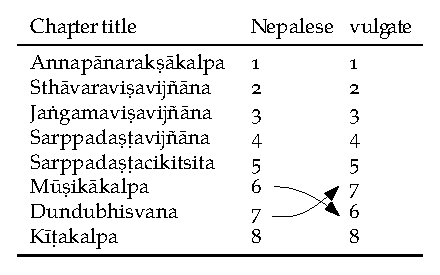
\includegraphics[width=0.65\linewidth]{chapters/media/kalpa}
%    \caption{}
%    \label{fig:kalpa}
%\end{figure}
%
\noindent
This difference in sequence does not have an immediately obvious 
significance, but it appears to be the most original known sequence of 
chapters, since it was already known to Jejjaṭa.\footnote{See note 
\ref{dalhana-rat-sequence} below.}

\section{The Spread of Indian Toxicological Lore to Medieval Islamic  
Authors}

\section{The \emph{Kalpasthāna}'s diffusion}

From the late eighth century onwards, the \emph{Kalpasthāna}, or parts
of it, began to circulate beyond the Indian subcontinent and to
influence medical literature in early Persia, Tibet and Cambodia.

In the late eighth century, the \emph{Kalpasthāna}, as part of the
\SS, was translated into Persian and Arabic at the Abbasid court of
Baghdad by an Indian physician who is often known by the name
Mankah.\footnote{On the name and its variants, see \volcite{IB}[202,
    notes 2, 3]{meul-hist}. For an account of this translation process see
    the account of \citet[14--18]{kahl-2015} and especially his useful
    reconstruction of likely historical events (16--17).}  The principle
    source of information about this translation is the \emph{ʿUyūn
        al-anbā' fī ṭabaqāt al-aṭibbā} of Ibn Abī Uṣaybiʿah
    (ca.\,1201--1270).\footnote{On Ibn ʿAbī Uṣaybʿiah, see
        \cite{hill-2019}. This author based his information on the earlier
        authors  Abū Ḥafṣ al-Kirmānī (fl.\,ca.\,800) and on an-Nadīm
        (d.\,990). Al-Kirmānī's treatise is unfortunately lost to history and
        known only through citations in other authors (see
        \cite{bosw-1994,blad-2011}).} Ibn Abī Uṣaybiʿah mentioned that al-Rāzī
        used the \SS, among other Indian works, and that it had been
        translated into Arabic at the orders of the Barmakid Yaḥyā ibn
        Khālid.\footnote{\volcite{3.2}[987]{sava-2019}. Ibn Abī Uṣaybiʿah said
            the work consisted of ten chapters, which does not match the six books
            of the known \SS.  He listed separately a work on poisonous snakes
            that could have been the \emph{Kalpasthāna} (\emph{ibid}, 989).  On
            the transmission of Sanskrit medical knowledge to Baghdad through the
            influence of the Barmakids, see
            \cites{blad-2011}{shef-2013}{kahl-2015}{wuja-2016a}.}  The \SS\
            passages used by al-Rāzī have been identified and printed in parallel
            with the Arabic translation by
            \citeauthor{kahl-2015}.\footnote{\cite[76--82]{kahl-2015}.
                Unfortunately, Kahl (p.\,14) accepted the impossible dating of a
                medical author Suśruta to the sixth century \BCE, in spite of citing
                \citeauthor{meul-hist}, \emph{HIML}, amongst his references. However,
                his remarks dating the redaction of the \SS\ to the period third-sixth
                century \CE\ are not incorrect.}
                
Ibn Abī Uṣaybiʿah gave a detailed description of the translation in
Baghdad of a work that was almost certainly the \emph{Kalpasthāna}:
\begin{quote}
Shānāq was the author of several books, notably: 1.\ On poisons, in
five parts. Mankah al-Hindī translated it from Sanskrit into Persian,
and a man by the name of Abū Ḥātim al-Balkhī was assigned the task of
transcribing it in Persian writing; he then expounded upon it to Yaḥyā
ibn Khālid ibn Barmak. The work was subsequently translated [into
Arabic] for the caliph al-Maʾmūn by his client, al-ʿAbbās ibn Saʿīd
al-Jawharī. The latter was also assigned the task of reading it aloud
to al-Ma’mūn.\fvolcite{3.2}[990]{sava-2019}
\end{quote}
There are several interesting features of this account, some of which
have been discussed elsewhere.\footnote{E.g., in the notes to the
    translation of \citeauthor{sava-2019}, in \volcite{IA}[352]{meul-hist}
    and elsewhere. It has not been remarked before that the interpreter
    Abū Ḥātim al-Balkhī was from Balkh, the original home of the Buddhist
    Barmakid family.}  As the pioneering work of \citeauthor{stra-1934}
    showed, the \emph{Poison Book} of “Shanaq” contained material directly
    translated from the first chapter of the
    \emph{Kalpasthāna}.\footnote{The passages cited by
        \citet[14--19]{stra-1934} include quite literal translations of
        \emph{Kalpasthāna} 1.37, 1.40, 1.42, 1.29--34cd, 1.47, 1.51cd--52,
        1.69, and the famous characterization of a poisoner at 1.19cd--23 (see
        above, p.\,\pageref{poisoner}).  The translator of this Arabic work
        may only have been aware of chapter 1 of the \emph{Kalpasthāna}.} The
        reception of these materials from the \SS\ under the name “Shanaq”
        remains a historical puzzle.\footnote{Most scholars agree that this is
            a Perso-Arabic reception of the Sanskrit name Cāṇakya, but that name
            was associated not with the \SS, but with the \emph{Arthaśāstra}
            during or after the time of the Gupta empire
            \citep[33--36]{oliv-2013}.  The suggestion that it may be “Śaunaka” is
            not supportable \volcite{1A}[150--152]{meul-hist}.} Several other
            Islamic authors knew and cited the \SS.\footnote{Listed with
                references in \volcite{1A}[352]{meul-hist}.}
                                
The \SS\ was also a formative source for later Arabic works on
toxicology.  One of the earliest mentions of Shanaq is made in ibn
Wahshiya's \emph{Book on Poisons} (ca.\,950). He refers to Shanaq's
book as great and important. This statement is attested to by the fact
that much of Shanaq's work was used by ibn
Wahshiya.\footcite[6]{leve-1966}
                                
The author Suśruta was also cited as a famous authority in Tibetan
lexicographical literature of the early ninth
century.\fvolcite{IA}[352]{meul-hist}
                                
Shortly after this time, inscriptional evidence by King Yaśovarman I
(r.\,889--910) shows that the \SS\ was known in
Cambodia.\footnote{\emph{Idem}.}
                                    
%In the eighth century, in Baghdad, portions of the \emph{Kalpasthāna}
% were translated into
% Arabic.\footnote{\cite{stra-1934}, \volcite{1}[]{meul-hist}}

%The \SS\ was translated into Persian or Arabic at the Abbasid court in
%the late eighth century by an Indian physician who is often known by
%the name Mankah.\footnote{On the name and its variants, see
%    \volcite{IB}[202, notes 2, 3]{meul-hist}.}  The principle source of
%    information about this translation is the 
%    \emph{ʿUyūn al-anbā' fī ṭabaqāt al-aṭibbā} of Ibn Abī Uṣaybiʿah, Aḥmad ibn 
%    al-Qāsim
%    (1201--1270):\footnote{On ʿAbī Uṣaybʿiah, see \cite{hill-2019}.}
%\begin{quote}
%    Mankah al-Hindī  was knowledgeable about the art of medicine,
%skilled in treating disease, and moderate in his methods; a
%philosopher of the previously mentioned group in the Indian
%sciences. He was also conversant with the Sanskrit and Persian
%languages: it was he who translated Shānāq’s \emph{On poisons}
%from Sanskrit to Persian. Mankah was a contemporary of Hārūn
%al-Rashīd, and during the latter’s caliphate he travelled from
%India to Iraq, where he met with the caliph and treated
%him.\footnote{Translation from
%    \volcite{3.2}[991--993]{sava-2019}.}
%\end{quote}
%`Abī Uṣayb`iah himself then went on to cite a passage that he relied on, taken 
%from  
%\emph{The History of the Caliphs and the Barmakids}  (\emph{Akhbār 
%al-Barāmikah}) written by  Abū Ḥafṣ 
%al-Kirmānī (fl.\ ca.\ 800).\footnote{This treatise is unfortunately lost to history 
%and 
%known only 
%through citations in other authors.   See further, \cite{bosw-1994,blad-2011}.}
%
%
%\volcite{IA}[352]{meul-hist}
%\cite{lang-2018}
%
%\citet[Introduction]{leve-1966} on 
%\begin{itemize}
%    \item translation of the \SS\ under the Barmakids (Pramukhas) in 
%    eighth-ninth-century Baghdad:
%    \begin{quote}
%        Much more important is the fact
%        that Mankah is known as the translator of the Susruta
%        samhita, a huge medical compendium, for Yahya b.~Khalid. Ibn abi Usaibi'a 
%        (1203/4--1270) also discussed
%        Mankah as an important Indian physician. Al-Jaiz
%        (d.\,868/9) knew of Mankah.'
%        \ldots
%        
%        Yahya ibn Khalid, a Barmecide, was famous in his
%        day in the field of science. In ibn al-Nadim, it is
%        related that Yah.ya sent a scholar to India to study
%        Indian drugs and religion, and brought Indian physi-
%        cians and philosophers westward so that he might learn
%        from them.
%        Caliph al-Ma'mfin  also was interested in the sci-
%        ences and so brought many scientists to his court from
%        Jundishapfir where there were not only Greek men of
%        science but also Indians who had brought their science
%        and wisdom.\footnote{\cite[6]{leve-1966}}
%    \end{quote}
%    
%    \item ibn Wahshiya's Book on Poisons (ca. 950). 
%    \begin{quote}
%        Not much is known of Shanaq himself. However,
%        what is one of the earliest mentions of him is made in
%        ibn Wahshiya's Book on Poisons (ca.\ 950). He refers
%        to Shanaq's book as great and important. This state-
%        ment is attested to by the fact that much of Shanaq's
%        work was used by ibn Wahshiya. It was not, however,
%        a base upon which the latter's work was built, as
%        Strauss has claimed.\footnote{Idem.}
%    \end{quote}
%    \item The Poison book of Cāṇakya.\footcite{stra-1934}
%
%\item The Poison Book of Maimonides (ca.\,1198 \CE):
%
%\citetitle{rosn-1968},\footcite{rosn-1968}  was written in
%approximately July 1198 at the request of his patron, al-Qadi
%al-Fadil (1135--1200) who served in Cairo under the Fatimid and
%Ayyubid administrations.\footcite[31]{krae-2005}
%\end{itemize}
